\documentclass[11pt]{article}
\usepackage[utf8]{inputenc}
\usepackage[T1]{fontenc}
\usepackage{lmodern}
\usepackage[a4paper,margin=2.4cm]{geometry}
\usepackage{amsmath,amssymb}
\usepackage{graphicx}
\usepackage{booktabs,longtable,array}
\usepackage[table]{xcolor}
\usepackage{caption}
\captionsetup{font=small,labelfont=bf,skip=4pt}
\usepackage[numbers,sort&compress]{natbib}
\usepackage{microtype}
\usepackage[hidelinks]{hyperref}
\usepackage{setspace}
\usepackage{lineno}
\usepackage{enumitem}
\setlist{itemsep=1pt,topsep=3pt}
\emergencystretch=3em
\onehalfspacing
\newcommand{\todo}[1]{\textcolor{red}{[#1]}}
\newcommand{\sig}{$^{*}$}

\title{\textbf{Protein language models complement, but do not replace, homology search for EC number prediction}\\[4pt]
\large A controlled comparison of embedding, structure and homology methods, including published predictors}
\author{Xiaoyu Zhang\\[2pt]\small\todo{Affiliation; corresponding author e-mail}}
\date{}

\begin{document}
\maketitle
\linenumbers

\begin{abstract}
\noindent Protein language model (PLM) embeddings and protein structure underpin most recent predictors of Enzyme
Commission (EC) numbers, but they are rarely compared with homology transfer under identical conditions. We compared
homology transfer by sequence (MMseqs2) and structure (Foldseek) search with classifiers on embeddings of seven PLMs,
two of them structure-aware, on sparse-autoencoder (SAE) features and on a fine-tuned PLM, and with their
combinations. We also re-ran seven published predictors (CLEAN, EnzHier, CLEAN-Contact, EnzymeHunter, MIL-BC+, MIL-CL+
and ESM2-BC). All methods used
the same 227,360 training enzymes and 5,242 EC numbers, were selected on a validation fold with at most 50\% identity
to training, and were scored once on six public test sets (3,394 enzymes) by per-enzyme F1. Homology transfer alone
averaged 0.604 over the test sets. The best single PLM embedding (ESM2-3B, 0.617) matched it without being
significantly better, SAE features tied it, and structure-aware PLMs (ProstT5, SaProt) and a fine-tuned ESMC fell
significantly below it. Structure helped through Foldseek search, not through structure-aware embeddings. PLM
classifiers and homology were complementary: classifiers were stronger on common ECs (0.90--0.92 vs 0.84), homology
on rare ECs and close homologues. An identity-gated blend of six PLM heads with sequence and structure homology scored
0.638, significantly better than homology alone on five of six sets. All seven published methods (0.503--0.574) fell
below homology alone, significantly on three to five sets each and even for queries with close training homologues,
and below the hybrid by up to 0.22.
Rankings also depended on the metric: the support-weighted F1 used in earlier benchmarks rewards over-calling and
reverses the reported advantage of MIL-BC+ over its sequence baseline. We recommend benchmarking EC predictors
against a sensitive homology baseline, with per-enzyme F1, calls per enzyme and paired bootstrap intervals.
\end{abstract}

\noindent\textbf{Keywords:} enzyme function prediction; EC number; protein language models; protein structure; homology
transfer; Foldseek; sparse autoencoders; benchmarking

% =====================================================================================================
\section{Introduction}

Enzyme Commission (EC) numbers are the standard four-level code for the reactions enzymes catalyse
\cite{mcdonald2023}. Most of the sequences in UniProt carry no experimentally supported function \cite{uniprot2025},
so EC numbers for new sequences are usually inferred, and doing so accurately is one of the most common tasks in
genome annotation.

The classical route is homology transfer: a query inherits the EC numbers of its closest annotated homologue.
Enzyme function is reliably conserved only above roughly 40--60\% sequence identity \cite{rost2002,tian2003}, and
transferred annotations propagate errors \cite{schnoes2009}. Two developments have nonetheless made homology transfer
much stronger than in early benchmarks. Sensitive search tools such as MMseqs2 find remote homologues at scale
\cite{mmseqs2}. Foldseek searches by structure, using a 3D-interaction (3Di) alphabet \cite{foldseek} that can be
computed from AlphaFold models of almost every UniProt protein \cite{jumper2021,afdb2022} or predicted directly from
sequence \cite{prostt5}.

Deep-learning EC predictors aim to go beyond homology. Early methods learned from sequence directly, using
convolutional networks (DeepEC \cite{deepec}), dilated residual networks (ProteInfer \cite{proteinfer}) or
transformer layers combined with homology search (DeepECtransformer \cite{deepectransformer}). Most recent methods
build on protein language model (PLM) embeddings, usually from ESM-1b or ESM2 \cite{esm1b,esm2}:
\begin{itemize}
  \item CLEAN learns a contrastive embedding and calls the nearest EC centroids \cite{clean}; EnzHier trains the same
        kind of embedding with a loss that follows the EC hierarchy \cite{enzhier}.
  \item CLEAN-Contact and EnzymeHunter add contact-map features \cite{cleancontact,enzymehunter}.
  \item GraphEC applies graph networks to ESMFold structures \cite{graphec}.
  \item MIL-BC treats a protein as a bag of structural domains and classifies it by multiple-instance learning
        \cite{milbc,dctdomain,ilse2018}.
\end{itemize}
Meanwhile the representations on offer have multiplied. They include larger sequence PLMs (ESM Cambrian, ESMC
\cite{esmc}; ProtT5 \cite{prottrans}), structure-aware PLMs that read 3Di tokens (ProstT5 \cite{prostt5}, SaProt
\cite{saprot}), and sparse autoencoders (SAEs) that decompose PLM activations into large dictionaries of interpretable
features \cite{gao2024sae,interplm,biohubsae}.

Whether any of these representations, or the published predictors built on them, predict EC numbers better than a
well-tuned homology search is not known.
Published comparisons differ in their training sets and EC vocabularies, in the decision rule that turns scores into
calls, in the averaging used for F1, and in whether a homology baseline is included at all. Several studies report the
support-weighted F1 of CLEAN's evaluation \cite{clean,milbc}, which, as we show, rewards calling extra ECs.
Benchmarks such as CARE \cite{care} fix the data splits but not the metric or the baselines. In related tasks,
simple homology baselines have proved hard to beat \cite{radivojac2013,zhou2019cafa}, and combining homology with
learned models has helped \cite{deepgoplus}.

Here we compare, under one protocol, homology transfer by sequence and structure search with classifiers on PLM
embeddings, SAE features and structure-aware PLMs, and with combinations of the two. We also re-run seven published EC
predictors on the same data. All methods share the training set, the EC vocabulary, the validation fold used for every
choice, the decision rule, the metric and six test sets (Fig.~\ref{fig:design}). We ask five questions:
\begin{enumerate}
  \item Does any PLM embedding or structure-based representation beat homology transfer alone?
  \item Where do learned models and homology succeed or fail, as a function of identity to training and of EC
        frequency?
  \item What is the best way to combine them?
  \item How do published deep-learning EC predictors compare with homology transfer and with these models?
  \item How does the choice of metric change the conclusions?
\end{enumerate}
In short, PLMs complement homology search but do not replace it. Single PLM embeddings, trained with a careful
recipe, match homology but do not beat it, and
structure-aware embeddings fall below it; structure helps through search instead. The two kinds of evidence are
complementary: PLMs are stronger on common ECs, homology on rare ones. Blending them, gated by the identity of the top
homologue, gives the best predictor we found. All seven published methods we re-ran fall below homology transfer
alone, significantly so on most test sets.

Our main contributions are:
\begin{enumerate}
  \item \textbf{A controlled comparison of representations against homology.} Embeddings from seven PLMs (two of
        them structure-aware), SAE features of two ESMC models and a partially fine-tuned PLM are each tested against
        sequence and structure homology transfer under the same protocol, with paired bootstrap intervals.
  \item \textbf{Structure is best used for search.} Foldseek search on AlphaFold or predicted 3Di improves on
        sequence search and on hybrids, whereas pooled structure-aware PLM embeddings fall below homology.
  \item \textbf{Where learned models and homology each win.} PLM classifiers are better on common ECs and homology on
        rare ones and close homologues. An analysis by identity to training and by EC frequency locates the remaining
        error.
  \item \textbf{A strong, simple hybrid.} Classifier probabilities are blended with homology transfer, gated by top-hit
        identity. It is significantly better than homology alone on five of six test sets.
  \item \textbf{A head-to-head re-evaluation of published methods.} CLEAN, EnzHier, CLEAN-Contact, EnzymeHunter,
        MIL-BC+, MIL-CL+ and ESM2-BC are re-run on the same training and test sets, and the re-runs reproduce the
        published scores of the first three. All seven fall below homology alone, including on close homologues,
        and below our hybrid on four or five sets each. We trace where and why: rare ECs, large EC classes for
        centroid-based methods, and calibration.
  \item \textbf{Negative results and a case for per-enzyme F1.} Structure-aware PLMs, model scale, head architecture,
        loss design, rare-class rebalancing and fine-tuning are reported with seed noise measured. Per-enzyme F1,
        reported with calls per enzyme, a homology baseline and paired bootstrap intervals, should replace
        support-weighted F1, which rewards over-calling and reverses published rankings.
\end{enumerate}

\begin{figure}[t]
\centering
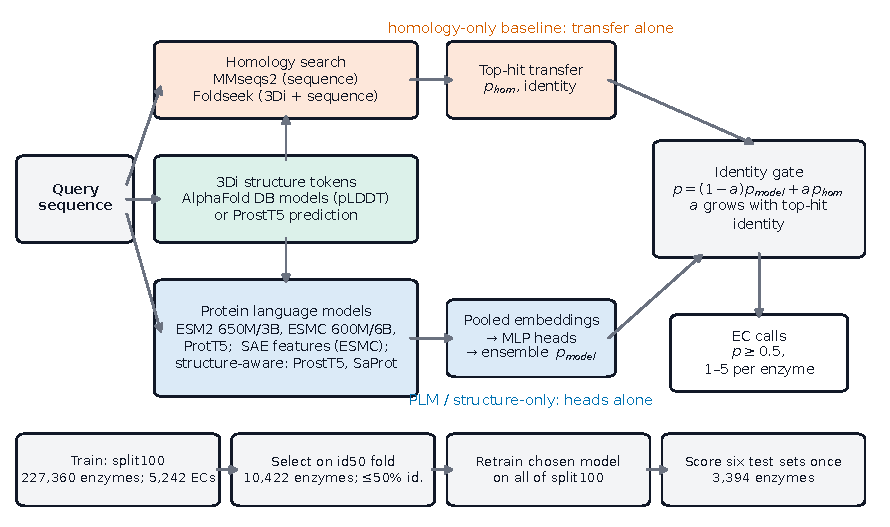
\includegraphics[width=\textwidth]{fig1_design.pdf}
\caption{\textbf{Study design.} Three families of evidence are compared: homology transfer from MMseqs2 (sequence) and
Foldseek (3Di structure tokens plus sequence) searches; classifiers on pooled embeddings of sequence PLMs, their
sparse-autoencoder (SAE) features and structure-aware PLMs; and identity-gated blends of the two. Every method uses the
same training set, decision rule and metric. All choices are made on the id50 validation fold, and the chosen
configuration is retrained on all training data and scored once on six test sets.}
\label{fig:design}
\end{figure}

% =====================================================================================================
\section{Results}

\subsection{A controlled benchmark of eight method categories}

All models were trained on split100, the 227,360-enzyme UniProt-derived training set of CLEAN \cite{clean,milbc},
with its vocabulary of 5,242 EC numbers. They were selected on id50, a fold of 10,422 split100 enzymes with no
training enzyme above 50\% identity at 50\% coverage. Final models were scored on six test sets (Table~\ref{tab:testsets}):
New-392 and Price-149 from CLEAN; UniProt-all and its multi-EC subset UniProt-multi; and Test-70 and Test-50, which pool
the others and remove queries within 70\% or 50\% identity of training \cite{milbc}. Every method calls ECs with
probability at least 0.5, with at least one and at most five calls per enzyme. The primary metric is per-enzyme F1,
the protein-centric F1 of CAFA \cite{radivojac2013,zhou2019cafa}. ``Test mean'' is the unweighted mean of the six
per-set scores.

\begin{table}[t]
\centering\small
\caption{\textbf{Test sets.}}
\label{tab:testsets}
\begin{tabular}{@{}lrrr@{}}
\toprule
test set & enzymes & ECs per enzyme & distinct ECs \\
\midrule
New-392 & 392 & 1.28 & 177 \\
Price-149 & 149 & 1.02 & 56 \\
UniProt-all & 987 & 1.09 & 488 \\
UniProt-multi & 77 & 2.16 & 110 \\
Test-70 & 1,057 & 1.11 & 492 \\
Test-50 & 732 & 1.06 & 339 \\
\bottomrule
\end{tabular}
\end{table}

We grouped about 180 trained models into eight categories (Supplementary Table~\ref{tab:all}):
\begin{itemize}
  \item \textbf{Homology only:} transfer from the top MMseqs2 or Foldseek hit, with no learned model.
  \item \textbf{Sequence PLM:} one MLP head on one pooled sequence-PLM embedding (ESM2-650M, ESM2-3B, ESMC-600M, ESMC-6B,
        ProtT5-XL).
  \item \textbf{PLM + SAE features:} the same head on max-pooled SAE features of ESMC.
  \item \textbf{Structure-aware PLM:} the same head on ProstT5 or SaProt embeddings.
  \item \textbf{Fine-tuned PLM:} ESMC-600M with its upper half fine-tuned.
  \item \textbf{PLM combination:} several embeddings, concatenated or ensembled, without homology.
  \item \textbf{PLM + homology:} PLM heads blended with homology transfer by an identity gate.
  \item \textbf{Published methods:} CLEAN \cite{clean}, EnzHier \cite{enzhier}, CLEAN-Contact \cite{cleancontact},
        EnzymeHunter \cite{enzymehunter}, ESM2-BC, MIL-BC+ and MIL-CL+ \cite{milbc}, re-run on the same test sets.
\end{itemize}
Figure~\ref{fig:categories} and Table~\ref{tab:best} compare the best model of each category on id50 and on the test
mean. Figure~\ref{fig:vshom} tests each against homology alone with paired bootstrap intervals.

\subsection{Homology transfer alone is a strong baseline}

Transfer from the top MMseqs2 hit scored 0.893 on id50 and 0.595 on the test mean (Supplementary
Table~\ref{tab:all}). Although id50 allows no training neighbour above 50\% identity, MMseqs2 still found
a hit at $e \leq 10^{-3}$ for 97.8\% of its queries, and for 87--97\% of test queries.

Searching by structure did better on the remote and out-of-distribution sets. Foldseek on ProstT5-predicted 3Di beat
MMseqs2 on Price-149 ($+0.039$), Test-50 ($+0.015$) and Test-70 ($+0.009$), and found a hit for 96--100\% of queries.
It was slightly worse on id50 (0.884), where amino-acid identity is the sharper signal. Real AlphaFold structures
raised Foldseek's id50 score (0.890 vs 0.884) but not its test mean (0.607 vs 0.608).

Combining the two searches without any learned model, by taking the calls of whichever tool's top hit has the higher
identity (``best hit''), gave the highest id50 of any homology-only method (0.897; test mean 0.604). Taking the union of
both tools' calls gave 0.894 and 0.608. Both lie within 0.004 of Foldseek alone and are not significantly different
from it. We use the id50-selected best-hit rule as the homology-only baseline. Homology transfer thus reaches
0.595--0.608 on the test mean, depending on the search. That is above every published method we re-ran (0.503--0.574;
Section~\ref{sec:published}).

\subsection{Single PLM embeddings match homology but do not beat it}

\begin{figure}[t]
\centering
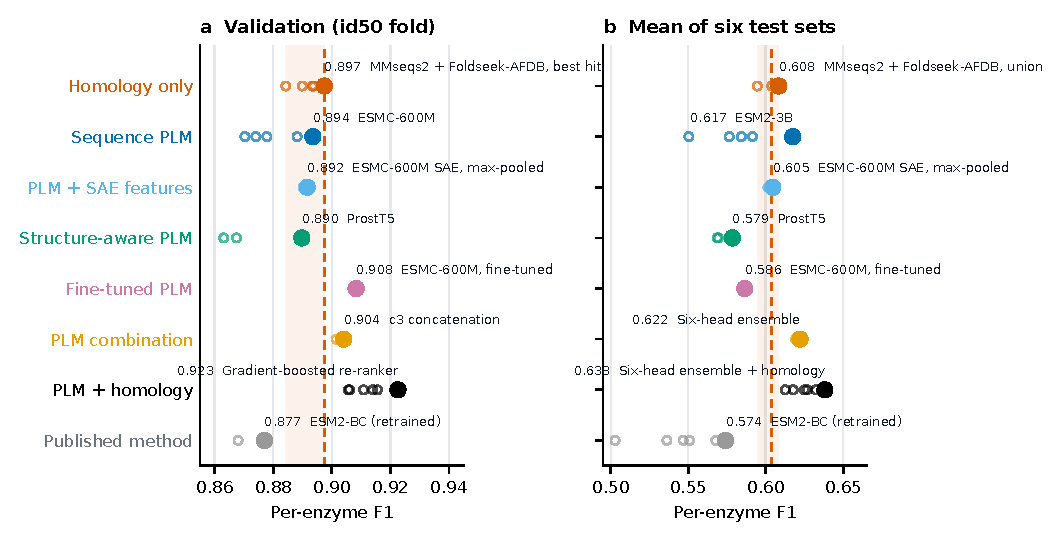
\includegraphics[width=\textwidth]{fig2_categories.pdf}
\caption{\textbf{Best model of each category on validation and test sets.} Per-enzyme F1 on the id50 validation fold
\textbf{(a)} and averaged over the six test sets \textbf{(b)}. Open circles are all models in a category; the filled
circle is the category's best on that axis, labelled with its score and name. The dashed line is the id50-selected
homology-only baseline (MMseqs2 + Foldseek-AFDB, best hit), and the shaded band spans all homology-only variants.
Published methods without an id50 score (MIL-CL+, EnzymeHunter, CLEAN, EnzHier, CLEAN-Contact) appear only in
\textbf{(b)}. Single-head scores are
three-seed means where seeds were run (Supplementary Table~\ref{tab:all}).}
\label{fig:categories}
\end{figure}

\begin{table}[t]
\centering\small
\caption{\textbf{Best model of each category.} Per-enzyme F1 on id50 and on each test set (full protocol). For each
category the row is the model with the highest test mean; where another model has the highest id50 it is listed
below in italics. $\Delta$hom is the test-mean difference from the id50-selected homology-only baseline (first row)
with its 95\% paired bootstrap interval; \sig\ marks intervals that exclude zero. $^{\dagger}$Mean of three seeds;
its $\Delta$hom uses seed 0.}
\label{tab:best}
\footnotesize\setlength{\tabcolsep}{2.6pt}
\begin{tabular}{@{}lrrrrrrrrl@{}}
\toprule
model & id50 & New & Price & U-all & U-multi & T-70 & T-50 & mean & $\Delta$hom [95\% CI] \\
\midrule
\multicolumn{10}{@{}l}{\textit{Homology only}}\\
\quad MMseqs2 + Foldseek-AFDB, best hit & .897 & .633 & .386 & .760 & .696 & .620 & .528 & .604 & -- \\
\quad \textit{MMseqs2 + Foldseek-AFDB, union} & .894 & .634 & .407 & .759 & .692 & .624 & .534 & .608 & $+.004$ [$-.001$,\,$.011$] \\
\multicolumn{10}{@{}l}{\textit{Sequence PLM}}\\
\quad ESM2-3B$^{\dagger}$ & .888 & .634 & .429 & .763 & .698 & .631 & .550 & .617 & $+.011$ [$-.004$,\,$.027$] \\
\quad \textit{ESMC-600M}$^{\dagger}$ & .894 & .572 & .413 & .739 & .698 & .589 & .494 & .584 & \\
\multicolumn{10}{@{}l}{\textit{PLM + SAE features}}\\
\quad ESMC-600M SAE, max-pooled$^{\dagger}$ & .892 & .607 & .420 & .760 & .678 & .621 & .541 & .605 & $+.000$ [$-.015$,\,$.015$] \\
\multicolumn{10}{@{}l}{\textit{Structure-aware PLM}}\\
\quad ProstT5 & .890 & .602 & .399 & .733 & .651 & .590 & .497 & .579 & $-.025$ [$-.041$,\,$-.009$]\sig \\
\multicolumn{10}{@{}l}{\textit{Fine-tuned PLM}}\\
\quad ESMC-600M, fine-tuned & .908 & .575 & .425 & .740 & .694 & .591 & .494 & .586 & $-.017$ [$-.033$,\,$-.002$]\sig \\
\multicolumn{10}{@{}l}{\textit{PLM combination}}\\
\quad Six-head ensemble & .901 & .613 & .437 & .772 & .728 & .632 & .552 & .622 & $+.018$ [$.005$,\,$.031$]\sig \\
\quad \textit{c3 concatenation} & .904 & .604 & .464 & .772 & .689 & .635 & .553 & .619 & $+.015$ [$.001$,\,$.028$]\sig \\
\multicolumn{10}{@{}l}{\textit{PLM + homology}}\\
\quad Six-head ensemble + homology & .914 & .640 & .425 & .787 & .751 & .653 & .574 & .638 & $+.034$ [$.025$,\,$.043$]\sig \\
\quad \textit{c3 + homology} & .916 & .636 & .440 & .783 & .716 & .650 & .570 & .632 & $+.029$ [$.017$,\,$.040$]\sig \\
\multicolumn{10}{@{}l}{\textit{Published method}}\\
\quad ESM2-BC (retrained) & .877 & .585 & .367 & .734 & .667 & .590 & .502 & .574 & \\
\bottomrule
\end{tabular}
\end{table}

With the same head and training recipe for every embedding, the best single PLM was ESM2-3B's final layer. Its test
mean over three seeds was 0.617 (range 0.613--0.624), with an id50 score of 0.888 (Fig.~\ref{fig:categories}). That is
$+0.011$ above homology alone on the test mean, an interval that includes zero [$-0.004$,\,$0.027$]. The difference was
not significant on any individual test set either (Fig.~\ref{fig:vshom}). The other sequence PLMs scored at or below
homology:
\begin{itemize}
  \item ESM2-650M: id50 0.878, test 0.592.
  \item ESMC-600M: id50 0.894, the highest of any frozen single embedding, but test 0.584.
  \item ProtT5-XL: 0.870 and 0.576.
  \item ESMC-6B: 0.874 and 0.550. Scale did not help pooled ESMC states.
\end{itemize}

Max-pooled SAE features were the best way to read ESMC. For ESMC-600M they reached 0.605 on the test mean, above
the final layer they are computed from (0.584), the mean-pooled SAE codes (id50 0.893 vs 0.881) and the SAE's
input layer (id50 0.893 vs 0.878). The 6B SAE gave 0.601. Max-pooling keeps the strongest residue-level feature
activations that a mean over the sequence dilutes. Even so, the best SAE head tied homology alone ($+0.000$
[$-0.015$,\,$0.015$]).

Fine-tuning the upper half of ESMC-600M (198M trainable parameters) gave the highest single-model id50 score (0.908).
On the tests, however, it scored 0.586, significantly below homology ($-0.017$ [$-0.033$,\,$-0.002$]).

\begin{figure}[t]
\centering
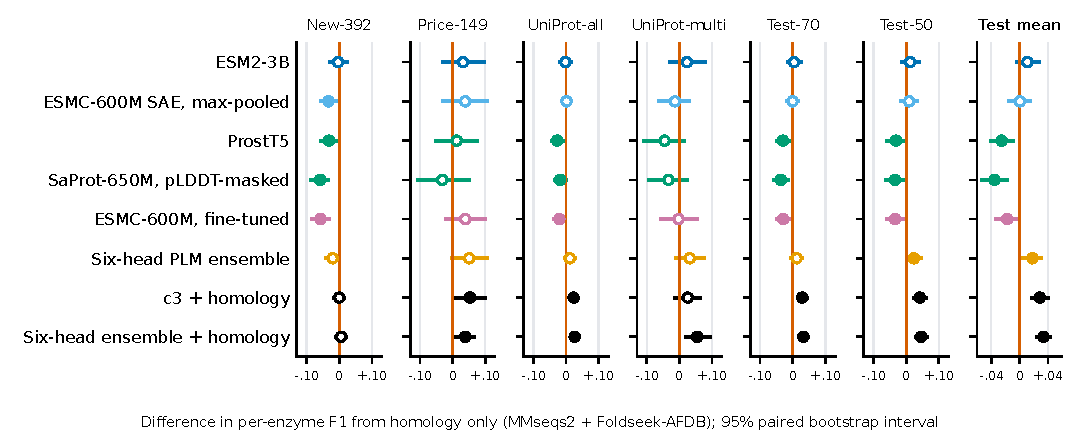
\includegraphics[width=\textwidth]{fig3_vs_homology.pdf}
\caption{\textbf{Learned models compared with homology alone, per test set.} Difference in per-enzyme F1 from the
homology-only baseline (MMseqs2 + Foldseek-AFDB, best hit; orange line), with 95\% paired bootstrap intervals (2,000
resamples). Filled markers exclude zero; open markers do not. Test-mean intervals average the six per-set differences
of each resample. Single heads are seed-0 runs.}
\label{fig:vshom}
\end{figure}

\subsection{Structure helps through search, not through structure-aware embeddings}
\label{sec:structure}

Structural information entered the comparison in three ways. Only search helped.
\begin{itemize}
  \item \textbf{Structure-aware embeddings fell below homology.} ProstT5 embeddings scored well on id50 (0.890,
        against 0.870 for their parent ProtT5) but only 0.579 on the tests, significantly below homology ($-0.025$).
        SaProt-650M scored 0.569 ($-0.035$), below even ESM2-650M (0.592), the sequence model it was initialised
        from.
  \item \textbf{SaProt does use its structure tokens.} With all 3Di tokens masked it fell to 0.464.
  \item \textbf{SaProt's recipe made no difference.} Masking 3Di states where AlphaFold pLDDT is below 70 left the
        test mean unchanged (0.569). It also left id50 within seed noise (0.863--0.879 vs 0.867--0.871 unmasked).
  \item \textbf{No gain at low identity.} Below 30\% identity, where structure should help most, pLDDT-masked SaProt
        scored 0.387 against 0.406 for ESM2-650M.
  \item \textbf{No gain in combination.} Added to the best concatenated head or to the best hybrid, SaProt tied
        (0.616 vs 0.619; 0.637 vs 0.638).
  \item \textbf{Structure search did help, in combination.} Adding Foldseek to the MMseqs2 gate raised the five-head
        hybrid from 0.628 to 0.636. Hybrids gated on both tools were significantly better than an MMseqs2-only hybrid
        (0.624) on Price-149, UniProt-all, Test-70 and Test-50.
\end{itemize}
The structural signal that pooled structure-aware embeddings carry appears to be captured more directly by searching
3Di sequences.

\subsection{Combining PLMs with homology gives the best predictor}

Combining embeddings without homology helped a little. Concatenating ESM2-3B, the ESMC-600M final layer and
ESMC-600M SAE-max into one head (``c3'') gave 0.619 ($+0.015$ over homology). An ensemble of six heads on different
embeddings gave 0.622 ($+0.018$). Both differences were significant on the test mean but on only one or two individual
sets (Fig.~\ref{fig:vshom}). At equal inputs, averaging separately trained heads beat a single concatenated head
(0.616 vs 0.604 for the ESM2-650M/ESMC-600M family).

Blending with homology helped much more. The hybrid mixes the ensemble probability with the homology call vector,
$p = (1-a)\,p_\text{model} + a\,p_\text{hom}$, using a weight $a$ that grows linearly with the identity of the top hit
(Methods). With both search tools in the gate:
\begin{itemize}
  \item every single-embedding head gained, by $+0.008$ to $+0.026$ on the test mean;
  \item the best single-embedding hybrids reached 0.625 (ESM2-3B) and 0.627 (ESMC-600M SAE);
  \item the c3 head reached 0.632, the highest id50 of any gated model (0.916);
  \item the six-head ensemble reached 0.638 (id50 0.914), $+0.034$ over homology alone [0.025, 0.043]. This gain was
        significant on five of six test sets, all but New-392 (Fig.~\ref{fig:vshom}).
\end{itemize}
Diversity mattered more under homology: one embedding against six gave 0.625--0.627 vs 0.638 with homology, but
0.617 vs 0.622 without it. Most of the six-head ensemble's advantage over the single-network hybrid came from
UniProt-multi (0.751 vs 0.716), where enzymes need two or more correct calls. On the other five sets the two tied.

A gradient-boosted re-ranker \cite{sklearn} over model and homology evidence, trained in place of the gate with
cross-validation folds grouped by 30\%-identity clusters, scored highest on id50 (0.923) but only 0.613 on the tests. It
learned the near-homologue regime that id50 over-represents (Section~\ref{sec:valtest}).

\subsection{PLMs and homology are complementary: identity and EC frequency}

Splitting the pooled test queries by top-hit identity to training (Fig.~\ref{fig:where}a) shows where each source of
evidence works:
\begin{itemize}
  \item \textbf{At 50\% identity or above}, homology alone scored 0.846--0.854. That matches the hybrid and beats
        every PLM head (0.805--0.846).
  \item \textbf{Between 30\% and 50\%}, the largest bin (1,519 queries), homology (0.586), ESM2-3B (0.580) and the
        six-head ensemble (0.591) were level. The hybrid scored 0.612.
  \item \textbf{Below 30\%}, the ensemble (0.465) beat homology (0.437), and the hybrid scored 0.483.
  \item \textbf{With no hit at all}, homology can only make an arbitrary call, while the ensemble still scored 0.404.
\end{itemize}

Splitting by the training count of the query's rarest EC (Fig.~\ref{fig:where}b) shows a sharper contrast:
\begin{itemize}
  \item \textbf{Common ECs (at least 200 training examples):} PLM classifiers scored 0.90--0.92 against 0.84 for
        homology. A classifier learns the full extent of a large class, while the nearest homologue often carries a
        different label.
  \item \textbf{Rare ECs (1--9 training examples):} homology scored 0.497, against 0.468 for ESM2-3B, 0.429 for ProstT5
        and 0.483 for the ensemble. With a handful of examples a classifier cannot learn an EC, whereas a single close
        homologue can still transfer it.
\end{itemize}
The identity gate exploits this division of labour. The hybrid was best or tied in every identity bin and in every
frequency bin.

The remaining error is concentrated where neither source works:
\begin{itemize}
  \item 85\% of the hybrid's error falls on queries below 50\% identity or with no hit;
  \item 48\% falls on queries whose EC has fewer than ten training examples, a third of all test queries
        (Fig.~\ref{fig:where}, bottom).
\end{itemize}

\begin{figure}[t]
\centering
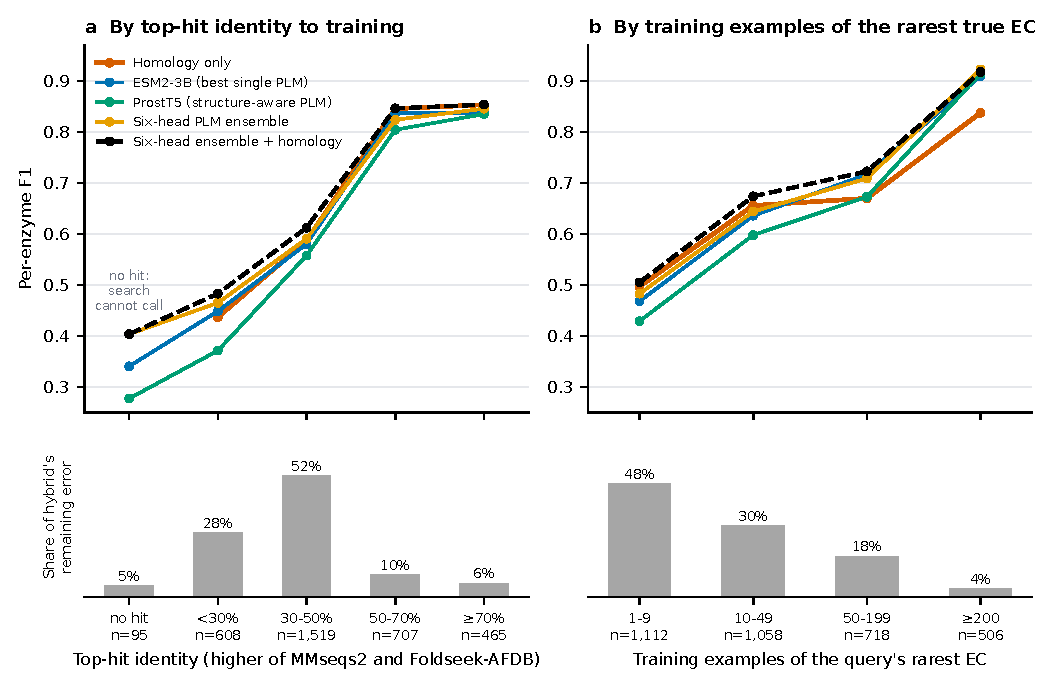
\includegraphics[width=\textwidth]{fig4_where.pdf}
\caption{\textbf{Where PLMs and homology succeed.} Per-enzyme F1 on the 3,394 pooled test queries \textbf{(a)} by
top-hit identity to training (the higher of MMseqs2 and Foldseek-AFDB) and \textbf{(b)} by the training count of the
query's rarest true EC. Bottom: each bin's share of the best hybrid's remaining error, $\sum_i (1 - F_{1,i})$. Homology
transfer is unavailable when no hit is found. Single heads are seed-0 full-protocol runs.}
\label{fig:where}
\end{figure}

\subsection{Published EC predictors fall below homology transfer}
\label{sec:published}

Most published deep-learning EC predictors are built on the same kinds of PLM embeddings we tested above. We asked
whether they, too, fall short of homology transfer, and how they compare with our models. We re-ran published methods
whose models could be applied to our test sets with the same EC vocabulary:
\begin{itemize}
  \item CLEAN \cite{clean}, EnzHier \cite{enzhier} and CLEAN-Contact \cite{cleancontact}, from their released split100
        models. All three learn a contrastive embedding and call ECs by max-separation over EC centroids. EnzHier adds a
        hierarchical loss; CLEAN-Contact replaces ESM-1b with ESM2-3B and adds a contact-map embedding of the
        AlphaFold or ESMFold structure;
  \item MIL-BC+ and MIL-CL+ \cite{milbc}, from their released checkpoints;
  \item ESM2-BC, the sequence baseline of \cite{milbc}, retrained by us because no checkpoint was released;
  \item EnzymeHunter \cite{enzymehunter} v0.1.15, whose reference set is identical to split100.
\end{itemize}
Each was scored from its prediction files with the same metric code as our models (Table~\ref{tab:published}). The
re-runs are faithful: under the support-weighted F1 used in \cite{milbc}, CLEAN and EnzHier matched the scores
reported there to within 0.001 on all six sets, and CLEAN-Contact did so on New-392 and both UniProt sets.

All seven fell below homology transfer alone. Their test means were 0.503--0.574, against 0.604 for the homology-only
baseline and 0.595 for MMseqs2 alone. In paired bootstrap tests, homology alone was significantly better than CLEAN,
EnzHier and MIL-CL+ on five test sets each, than EnzymeHunter, MIL-BC+ and ESM2-BC on four each and than
CLEAN-Contact on three, and it was never significantly worse on any set. Even plain MMseqs2 transfer was significantly
better than each published method on two to five sets. The sets that did not separate were mostly Price-149, whose 149
enzymes give 95\% intervals about 0.15 wide, and, against EnzymeHunter and CLEAN-Contact, New-392.

Our own learned models widened the gap. A single ESM2-3B head was significantly better than each published method on
four or five sets. The best hybrid was significantly better than CLEAN, EnzHier, MIL-BC+, MIL-CL+ and ESM2-BC on five
sets each and than EnzymeHunter and CLEAN-Contact on four. Against these two, every model of ours tied on New-392 and
Price-149, the two sets inherited from CLEAN, and was better on the four newer sets, by up to 0.16.

The three CLEAN-family methods form a controlled series: same training set, contrastive objective and decision rule.
\begin{itemize}
  \item \textbf{Hierarchical loss.} EnzHier scored below CLEAN (0.503 vs 0.536), significantly on three sets.
  \item \textbf{Larger PLM and structure.} CLEAN-Contact scored above CLEAN (0.568 vs 0.536), significantly on three
        sets, and was the best centroid-based method. It still fell below homology alone (0.604) and below a plain MLP
        head on the same ESM2-3B embedding without any structure (0.615), significantly on four sets. As for the
        structure-aware PLMs (Section~\ref{sec:structure}), structure added to an embedding gained less than the
        choice of head and decision rule.
\end{itemize}

Splitting the pooled test queries as in Fig.~\ref{fig:where} shows where the published methods fall short
(Fig.~\ref{fig:published}). They share the weaknesses of our PLM heads, but more severely:
\begin{itemize}
  \item \textbf{Close homologues.} At 50\% identity or more, homology transfer scored 0.846--0.854, our PLM heads
        0.805--0.846 and the published methods 0.70--0.82. A classifier that ignores its nearest training neighbour gives
        up the most reliable evidence available.
  \item \textbf{Rare ECs.} For ECs with 1--9 training examples, homology scored 0.497, our PLM heads
        0.43--0.48 and the published methods 0.40--0.46.
  \item \textbf{Large EC classes, for centroid-based methods.} On ECs with at least 200 training examples the two
        classifiers beat homology (ESM2-BC 0.895, MIL-BC+ 0.878, homology 0.838), as our heads did (0.90--0.92). All five
        contrastive, centroid-based methods did not (0.62--0.79: EnzymeHunter 0.622, EnzHier 0.649, CLEAN 0.750,
        MIL-CL+ 0.785, CLEAN-Contact 0.793). One centroid cannot represent a large EC class that spans unrelated
        families; our own prototype output layer failed the same way (Supplementary Table~\ref{tab:negative}).
  \item \textbf{No hit.} Only for the 95 queries without a homologue did the published methods (0.28--0.41) add
        something homology cannot.
\end{itemize}
Calibration and training recipe also matter. Released MIL-BC+ makes 1.63 calls per enzyme, more than any other method
(1.17--1.39), which costs it precision under per-enzyme F1 (Section~\ref{sec:metric}). With the same ESM2-650M
embedding as ESM2-BC, our head and training recipe scored 0.592 against 0.574.

Other recent methods could not be placed in this comparison, including DeepECtransformer \cite{deepectransformer} and
GraphEC \cite{graphec}. Their published numbers use different training data, decision rules or F1 averaging, so copying
them into Table~\ref{tab:published} would mix protocols and metrics.

\begin{table}[t]
\centering\small
\caption{\textbf{Published methods against homology and this study.} Top: per-enzyme F1 on the six test sets, its
mean, the means of micro and support-weighted F1, and mean calls per enzyme. Bottom: paired bootstrap differences in
per-enzyme F1 (2,000 resamples). \sig\ 95\% interval excludes zero. $^{\ddagger}$Seed-0 run (three-seed mean 0.617).}
\label{tab:published}
\footnotesize\setlength{\tabcolsep}{2.9pt}
\begin{tabular}{@{}lrrrrrrrrrr@{}}
\toprule
method & New & Price & U-all & U-multi & T-70 & T-50 & mean & micro & weighted & calls \\
\midrule
CLEAN & .535 & .424 & .679 & .580 & .542 & .458 & .536 & .525 & .539 & 1.23 \\
EnzHier & .522 & .417 & .635 & .533 & .500 & .409 & .503 & .487 & .508 & 1.25 \\
CLEAN-Contact & .619 & .422 & .688 & .595 & .583 & .499 & .568 & .551 & .557 & 1.20 \\
EnzymeHunter & .620 & .416 & .656 & .596 & .539 & .453 & .547 & .530 & .557 & 1.29 \\
MIL-CL+ (released) & .575 & .402 & .695 & .591 & .562 & .480 & .551 & .533 & .553 & 1.31 \\
MIL-BC+ (released) & .560 & .397 & .713 & .684 & .578 & .500 & .572 & .545 & .614 & 1.63 \\
ESM2-BC (retrained) & .585 & .367 & .734 & .667 & .590 & .502 & .574 & .568 & .548 & 1.18 \\
\addlinespace
Homology, MMseqs2 & .622 & .385 & .754 & .684 & .610 & .514 & .595 & .572 & .593 & 1.34 \\
Homology, best hit & .633 & .386 & .760 & .696 & .620 & .528 & .604 & .574 & .602 & 1.39 \\
ESM2-3B head$^{\ddagger}$ & .629 & .418 & .758 & .719 & .624 & .540 & .615 & .610 & .596 & 1.18 \\
Six-head ensemble & .613 & .437 & .772 & .728 & .632 & .552 & .622 & .616 & .599 & 1.17 \\
Best hybrid & \textbf{.640} & .425 & \textbf{.787} & \textbf{.751} & \textbf{.653} & \textbf{.574} & \textbf{.638} & \textbf{.625} & \textbf{.620} & 1.24 \\
\midrule
homology $-$ CLEAN & $+.098$\sig & $-.037$ & $+.082$\sig & $+.116$\sig & $+.078$\sig & $+.070$\sig & & & & \\
homology $-$ EnzHier & $+.111$\sig & $-.031$ & $+.125$\sig & $+.163$\sig & $+.120$\sig & $+.119$\sig & & & & \\
homology $-$ CLEAN-Contact & $+.013$ & $-.035$ & $+.072$\sig & $+.101$\sig & $+.038$\sig & $+.029$ & & & & \\
homology $-$ EnzymeHunter & $+.013$ & $-.030$ & $+.104$\sig & $+.100$\sig & $+.081$\sig & $+.075$\sig & & & & \\
homology $-$ MIL-CL+ & $+.058$\sig & $-.015$ & $+.065$\sig & $+.105$\sig & $+.058$\sig & $+.048$\sig & & & & \\
homology $-$ MIL-BC+ & $+.073$\sig & $-.010$ & $+.047$\sig & $+.012$ & $+.042$\sig & $+.028$\sig & & & & \\
homology $-$ ESM2-BC & $+.048$\sig & $+.019$ & $+.026$\sig & $+.029$ & $+.030$\sig & $+.026$\sig & & & & \\
\addlinespace
hybrid $-$ CLEAN & $+.105$\sig & $+.001$ & $+.108$\sig & $+.170$\sig & $+.110$\sig & $+.117$\sig & & & & \\
hybrid $-$ EnzHier & $+.118$\sig & $+.008$ & $+.151$\sig & $+.217$\sig & $+.153$\sig & $+.166$\sig & & & & \\
hybrid $-$ CLEAN-Contact & $+.020$ & $+.003$ & $+.098$\sig & $+.155$\sig & $+.070$\sig & $+.075$\sig & & & & \\
hybrid $-$ EnzymeHunter & $+.019$ & $+.009$ & $+.130$\sig & $+.155$\sig & $+.114$\sig & $+.121$\sig & & & & \\
hybrid $-$ MIL-CL+ & $+.065$\sig & $+.023$ & $+.091$\sig & $+.160$\sig & $+.090$\sig & $+.094$\sig & & & & \\
hybrid $-$ MIL-BC+ & $+.080$\sig & $+.028$ & $+.074$\sig & $+.067$\sig & $+.075$\sig & $+.074$\sig & & & & \\
hybrid $-$ ESM2-BC & $+.055$\sig & $+.058$ & $+.052$\sig & $+.084$\sig & $+.062$\sig & $+.073$\sig & & & & \\
\bottomrule
\end{tabular}
\end{table}

\begin{figure}[t]
\centering
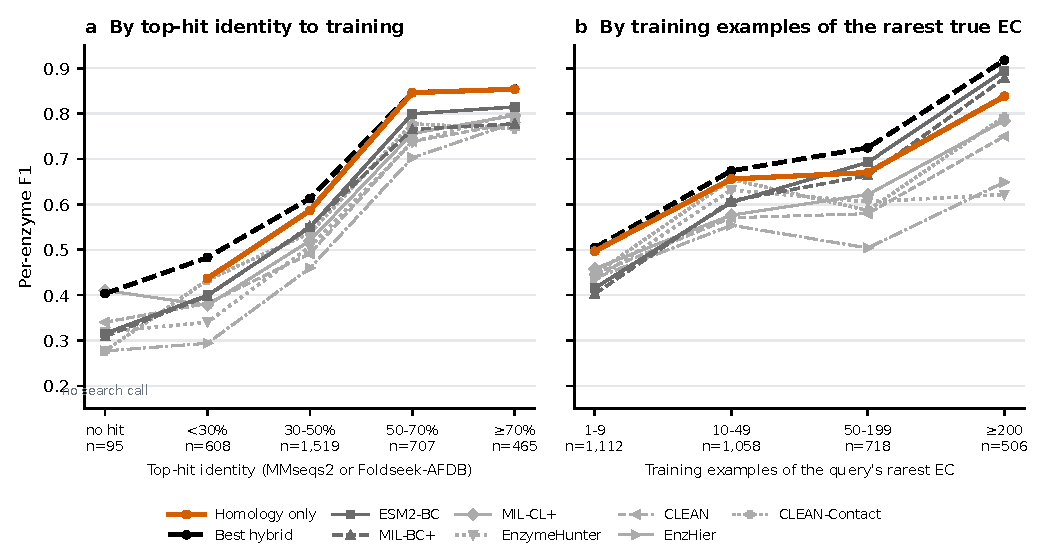
\includegraphics[width=\textwidth]{fig5_published.pdf}
\caption{\textbf{Where published methods fall short of homology.} Per-enzyme F1 on the 3,394 pooled test queries
\textbf{(a)} by top-hit identity to training (the higher of MMseqs2 and Foldseek-AFDB) and \textbf{(b)} by the training
count of the query's rarest true EC. Grey: published methods re-run on our test sets, dark for the two classifiers
(ESM2-BC, MIL-BC+) and light for the five contrastive, centroid-based methods. Homology transfer cannot call when no
hit is found.}
\label{fig:published}
\end{figure}

\subsection{Validation on id50 only partly predicts test performance}
\label{sec:valtest}

Across the 26 models with an id50 score, id50 and the test mean were correlated (Spearman $\rho = 0.81$;
Fig.~\ref{fig:idtest}). Among the 18 models with id50 at least 0.885, however, the correlation fell to 0.60, and
several of them were ranked very differently:
\begin{itemize}
  \item the re-ranker had the highest id50 (0.923) but a test mean of only 0.613;
  \item fine-tuned ESMC-600M had the highest single-model id50 (0.908) but tested at 0.586;
  \item frozen ESMC-600M scored 0.894 on id50 but 0.584 on the tests;
  \item ESM2-3B, the best single embedding on the tests (0.617), ranked behind ESMC-600M on id50 (0.888).
\end{itemize}

The id50 fold is drawn from the training distribution. Of its queries, 89\% have their top hit at 30--50\% identity,
and 48\% carry a common EC (at least 200 training examples), against 15\% of test queries. Within the same 30--50\%
identity bin, homology scored 0.926 on id50 but 0.586 on the tests. id50 therefore rewards fitting common classes and
near-homologue structure, and barely registers gains on rare or newly annotated ECs.

\begin{figure}[t]
\centering
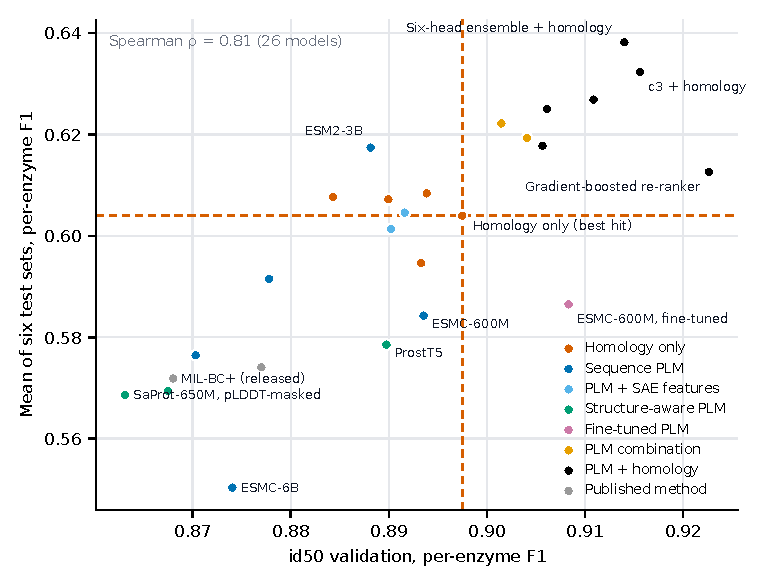
\includegraphics[width=0.75\textwidth]{fig6_id50_vs_test.pdf}
\caption{\textbf{Validation and test performance.} id50 validation F1 against the test mean for every model with an
id50 score, coloured by category. Dashed lines mark the homology-only baseline. Models to the right of the vertical
line and below the horizontal line, such as the re-ranker and fine-tuned ESMC-600M, look better than homology on
validation but not on the tests.}
\label{fig:idtest}
\end{figure}

\subsection{The choice of metric changes the conclusions}
\label{sec:metric}

CLEAN's evaluation \cite{clean}, reused by \cite{milbc}, computes F1 per EC and averages over the ECs present in the
test set's truth, weighted by their support. An EC that never occurs in a test set's truth gets zero weight, so a false
call on it costs nothing. In the MIL-BC models, 39--51\% of calls beyond the top-ranked EC fell on such zero-weight
ECs, and the support-weighted F1 rose monotonically as the decision threshold was lowered.

Figure~\ref{fig:metrics} shows the consequence. Shifting the logits of ESM2-BC or retrained MIL-BC+ by $+5$, the
shift that maximises support-weighted F1 on id50, raised their calls from 1.2 to 2.5 per enzyme. Their weighted F1
rose from 0.548--0.562 to 0.638--0.639, while their per-enzyme F1 fell from 0.567--0.574 to 0.501--0.509. Under the
weighted metric these over-calling models would outrank our best hybrid (0.620), which is better by 0.06--0.14 on
per-enzyme F1. The released MIL-BC+ makes 1.63 calls per enzyme, more than the retrained copy (1.20) or ESM2-BC (1.18).
Under weighted F1 it beat ESM2-BC on all six sets (Test-70 $+0.039$, significant). Under per-enzyme or micro F1 it was
significantly better on none, and significantly worse on UniProt-all ($-0.021$). The reported advantage of
domain-based MIL over the sequence baseline is therefore largely a calibration effect of the metric.

The comparison of published methods with homology depends on the metric too (Table~\ref{tab:published}). Under
per-enzyme F1, homology alone beats all seven. Under micro F1 it still beats CLEAN, EnzHier, MIL-CL+, EnzymeHunter and
released MIL-BC+ on three to five sets each and CLEAN-Contact on two, but ties ESM2-BC on every set. Under support-weighted F1, released MIL-BC+ (0.614) ranks
above homology alone (0.602), the single ESM2-3B head (0.596) and the six-head ensemble (0.599), second only to the best
hybrid (0.620). Its extra calls are charged under the other two metrics but not under this one.

\begin{figure}[t]
\centering
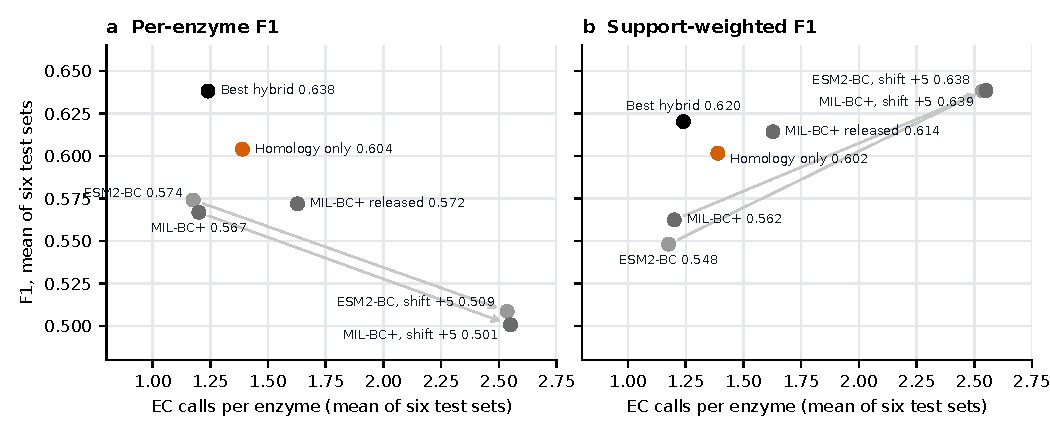
\includegraphics[width=\textwidth]{fig7_metrics.pdf}
\caption{\textbf{Support-weighted F1 rewards over-calling.} Mean over six test sets of \textbf{(a)} per-enzyme F1 and
\textbf{(b)} support-weighted F1, against calls per enzyme. Arrows show the effect of the logit shift ($+5$) chosen on
id50 to maximise support-weighted F1. It more than doubles the calls, lowers per-enzyme F1 and raises weighted F1
above that of the best hybrid.}
\label{fig:metrics}
\end{figure}

\subsection{Most modelling choices are within seed noise}

We measured seed noise directly by retraining all six ensemble members with three seeds on both protocols. Single heads
moved by up to 0.01 on the test mean and Price-149 alone by 0.02, while the hybrid moved by about 0.003 (0.635--0.638).
Against that noise, none of the interventions in Supplementary Table~\ref{tab:negative} improved the hybrid:
\begin{itemize}
  \item deeper and residual heads and a transformer over embedding blocks;
  \item asymmetric, focal and EC-hierarchy losses;
  \item rare-class loss reweighting and logit adjustment \cite{menon2021};
  \item cosine and prototype output layers \cite{snell2017};
  \item nearest-neighbour transfer in embedding space \cite{littmann2021,schutze2022};
  \item averaging seeds.
\end{itemize}
Since the first hybrid gated on both MMseqs2 and Foldseek, every hybrid has scored 0.913--0.916 on id50 and 0.633--0.642
on the tests.

% =====================================================================================================
\section{Discussion}

\paragraph{PLM embeddings have not yet replaced homology search.}
Under a common protocol, no single PLM embedding, SAE dictionary or structure-aware PLM beat homology transfer from
MMseqs2 and Foldseek, and the structure-aware embeddings fell below it. This does not mean the embeddings are
uninformative. A PLM head and a homology search reach similar overall accuracy through different routes:
\begin{itemize}
  \item the classifier learns the extent of well-populated EC classes, including members whose nearest homologue
        carries another label;
  \item search transfers rare labels that no classifier can learn from a handful of examples.
\end{itemize}
The identity-gated blend is a simple way to use both. It trusts homology in proportion to the identity of the top hit
and lets the model fill in where hits are weak or missing. A similar division between sequence-similarity and learned
components has been reported for GO prediction \cite{deepgoplus}. Our results suggest that new EC predictors should be
benchmarked against such hybrids, not only against other learned models.

\paragraph{Structure.}
Structure added value when used for search. Foldseek improved on MMseqs2 for the remote and out-of-distribution sets,
and adding it to the gate gave significant gains on four sets. Frozen, pooled embeddings from structure-aware PLMs did
not. A pooled embedding is dominated by the confident core of a protein, whose structural signal may already be
implied by its sequence. Search, by contrast, aligns residues and so uses local structural similarity directly. SaProt's
published EC gains come from fine-tuning \cite{saprot}, which we did not attempt. The difference between real
AlphaFold and ProstT5-predicted 3Di was small, and it was negative for Price-149, whose queries have only predicted
3Di but were searched against real-structure targets.

\paragraph{Published methods fall short of a homology baseline.}
The same comparison applied to published predictors is starker. The seven we could re-run, all built on PLM
embeddings and several also on contact maps, scored below homology transfer alone, significantly so on most test sets, and
below our hybrid. Three reasons emerge from where they fail:
\begin{itemize}
  \item \textbf{They do not use the nearest neighbour.} They lose most to homology where a close training homologue
        exists (at least 50\% identity) and on rare ECs, where a classifier has too few examples to learn from but a
        single homologue can still transfer the label.
  \item \textbf{Centroids do not fit large classes.} The five contrastive methods represent each EC by one centroid,
        which fails for large classes that span several families. They scored 0.62--0.79 on ECs with at least 200
        training examples, against 0.84 for homology and 0.88--0.92 for classifiers. Neither a hierarchical loss
        (EnzHier) nor a structure embedding (CLEAN-Contact) removed this gap.
  \item \textbf{Calibration.} Released MIL-BC+ over-calls, which the support-weighted F1 used in its evaluation
        rewards.
\end{itemize}
Evaluations that omit a sensitive homology baseline, or use a metric that does not charge false calls, can therefore
report progress that does not hold against simple transfer. Such a baseline should be the first row of any EC
benchmark.

\paragraph{Why predictions fail.}
The remaining error has four sources:
\begin{itemize}
  \item \textbf{Remote, rare queries.} Most of the error falls on queries that are both distant from training and
        carry rare ECs. There, neither a close homologue nor enough training examples exist. Rebalancing did not help:
        neither loss reweighting nor logit adjustment moved the rare tail, and a prototype layer helped rare ECs
        slightly (0.489 vs 0.458) but broke common ones. The gap is therefore not a class-prior bias. A handful of
        training proteins does not place remote members of the same EC near them in embedding space.
  \item \textbf{Close homologues with a different EC.} On New-392, queries with at least 70\% identity to a training
        enzyme score only 0.709. Recently annotated enzymes often carry a refined or different EC from their close
        homologues; function can diverge even at high identity \cite{rost2002,tian2003}; and some training labels are
        themselves transferred and possibly wrong \cite{schnoes2009}. No similarity-based method can recover these
        cases.
  \item \textbf{Enzymes with several ECs.} These need several correct calls, and a fixed 0.5 threshold with a one-call
        floor favours single calls. Diverse ensembles helped most here (UniProt-multi 0.751 vs 0.716).
  \item \textbf{Out-of-distribution sets.} Price-149 consists of bacterial proteins annotated from mutant phenotypes
        \cite{price2018}, and homology misleads there. The c3 head alone (0.464) beat both its own hybrid (0.440) and
        the best hybrid (0.425).
\end{itemize}

\paragraph{Choosing the metric.}
EC prediction is multi-label (1.02--2.16 ECs per enzyme here), long-tailed (5,242 ECs) and thresholded. The metric
must charge every false call, or calibration differences masquerade as model differences. We recommend:
\begin{enumerate}
  \item \textbf{Per-enzyme F1 as the primary metric.} It is protein-centric, as in CAFA \cite{radivojac2013,zhou2019cafa},
        and matches the use case of annotating one protein at a time.
  \item \textbf{Calls per enzyme reported next to every F1.}
  \item \textbf{Micro F1 as a secondary check}, with Fmax only as a threshold-free ranking.
  \item \textbf{F1 by EC frequency or by identity to training} for the hard regimes (Fig.~\ref{fig:where}).
  \item \textbf{Thresholds and every other choice made on validation data}, never on the tests.
  \item \textbf{Paired bootstrap intervals and seed replicates.} Price-149 and UniProt-multi have 95\% intervals about
        0.15 wide, and single heads vary by up to 0.01 between seeds.
  \item \textbf{A sensitive homology-only baseline} under the same metric.
\end{enumerate}
Averages over test sets weight a 77-enzyme set equally with a 1,057-enzyme set, and Test-70 and Test-50 are drawn from
the other sets. We report the test mean for convenience, but significance should be judged per set.

\paragraph{Limitations.}
\begin{itemize}
  \item \textbf{One training set and vocabulary.} All results use split100 and its 5,242 ECs. Out-of-vocabulary ECs,
        incomplete EC numbers and non-enzymes were not considered, and EnzymeHunter was run without its
        enzyme/non-enzyme filter. The released CLEAN-Contact model was trained on the 98.8\% of split100 with an
        AlphaFold structure, and 196 of its test queries used ESMFold rather than AlphaFold structures; its Price-149
        score (0.452 support-weighted) is below the 0.478 reported with the authors' own predicted structures
        \cite{milbc}.
  \item \textbf{Small, overlapping test sets.} Five New-392 sequences are identical to training sequences, for every
        method.
  \item \textbf{Labels taken as ground truth.} Part of the measured error is annotation change or error.
  \item \textbf{Possible leakage through pre-training.} PLMs and AlphaFold DB were built from UniProt releases that may
        include test sequences, though not their EC labels. Homology databases were restricted to each protocol's
        training set.
  \item \textbf{Frozen, pooled embeddings and simple heads.} Only ESMC-600M was fine-tuned, and only its upper half.
        Other recipes, including fine-tuned structure-aware PLMs or residue-level models, may change the PLM rows.
  \item \textbf{Simple homology rules.} We used top-hit transfer with a bit-score tolerance. More elaborate rules, such
        as weighting several hits, could strengthen the homology baseline further.
  \item \textbf{Selection on id50,} a fold that under-represents remote and rare queries (Section~\ref{sec:valtest}).
  \item \textbf{Single seeds} for most comparisons outside the main ensemble members.
\end{itemize}

\paragraph{Conclusions.}
PLM embeddings complement, but do not replace, a sensitive homology search by sequence and structure. Under
one protocol, PLM embeddings, SAE features and structure-aware PLMs on their own match but do not beat that search. The two kinds of evidence are complementary: PLM classifiers
handle common ECs, and homology handles rare ECs and close homologues. An identity-gated blend of diverse PLM heads
with sequence and structure search is significantly better than either alone. Structure helps through search rather
than through embeddings. Seven published deep-learning EC predictors, re-run under the same protocol, fall below
homology search alone, most clearly on close homologues and rare ECs, so a homology baseline belongs in every EC
benchmark. The open problem is the remote, rare regime, which current validation folds barely measure. Progress there
will need validation sets that resemble new annotations, by time or by EC frequency, and models that can learn an EC
from few examples, such as residue-level models of active sites or reaction-aware representations \cite{care}.

% =====================================================================================================
\section{Methods}

\subsection{Data}

\paragraph{Training set.} All models used split100, CLEAN's UniProt-derived training set \cite{clean}, as distributed
with \cite{milbc}. Sequences shorter than five residues were dropped, leaving 227,360 enzymes and 5,242 EC numbers.

\paragraph{Test sets.} We used the six test sets of \cite{milbc} (Table~\ref{tab:testsets}):
\begin{itemize}
  \item \textbf{New-392 and Price-149} come from CLEAN \cite{clean}. Price-149 derives from mutant-phenotype data
        \cite{price2018} and has RefSeq identifiers.
  \item \textbf{UniProt-all} holds enzymes deposited in UniProt between May 2022 and October 2025, and UniProt-multi
        is its subset with more than one EC.
  \item \textbf{Test-70 and Test-50} pool the other sets and remove every query that clusters with training at 70\% or
        50\% identity.
\end{itemize}


\subsection{Protocol}
Every choice was made on the id50 validation fold and never on the test sets. This covers features, head, loss,
epochs, ensemble members, gate parameters, homology combination rule and decision threshold.
\begin{itemize}
  \item \textbf{id50 fold.} 10,422 split100 enzymes clustered by identity. Training enzymes with more than 50\% identity
        at 50\% coverage to any fold member were excluded, leaving 204,558 for training.
  \item \textbf{Full protocol.} The chosen configuration was retrained on all of split100, with homology databases
        rebuilt on it, and scored once on the six test sets.
  \item \textbf{Hardware.} Two NVIDIA RTX A6000 GPUs.
\end{itemize}

\subsection{Representations}
Each protein is represented by one fixed-length vector per representation: the mean over residues of a chosen layer,
excluding special tokens (Table~\ref{tab:reps}). SAE features were also max-pooled, then transformed by log1p.

\paragraph{SaProt input.} SaProt reads one token per residue that combines the amino acid with a 3Di state.
\begin{itemize}
  \item \textbf{3Di source.} 3Di came from AlphaFold DB Swiss-Prot models (v6) \cite{afdb2022} when the accession had a
        model with an identical sequence. This covers 98.7\% of training proteins, 85--99\% of the UniProt-derived test
        sets and none of Price-149. Other proteins used ProstT5-predicted 3Di \cite{prostt5}.
  \item \textbf{pLDDT masking.} Following \cite{saprot}, 3Di states with pLDDT below 70 were masked: 5.9\% of AFDB
        residues, read from the B-factor column of the model files.
  \item \textbf{Control.} A sequence-only control masked all 3Di states.
\end{itemize}

\begin{table}[t]
\centering\small
\caption{\textbf{Representations.}}
\label{tab:reps}
\footnotesize
\begin{tabular}{@{}llrl@{}}
\toprule
representation & layer(s) & dim. & notes \\
\midrule
ESM2-650M \cite{esm2} & final & 1,280 & embedding of ESM2-BC and MIL-BC+ \cite{milbc} \\
ESM2-3B \cite{esm2} & final; layer 24 & 2,560 & fp16 \\
ESMC-600M \cite{esmc} & final; layer 27 & 1,152 & bf16 \\
ESMC-6B \cite{esmc} & final; layer 60 & 2,560 & \\
ESMC-600M SAE \cite{biohubsae} & layer-27 TopK-64 codes & 16,384 & mean- or max-pooled, log1p \\
ESMC-6B SAE \cite{biohubsae} & layer-60 TopK-64 codes & 16,384 & as above \\
ProtT5-XL-U50 \cite{prottrans} & encoder & 1,024 & fp16 \\
ProstT5 \cite{prostt5} & encoder (AA$\to$3Di prefix) & 1,024 & also predicts 3Di \\
SaProt-650M-AF2 \cite{saprot} & final; layer 24 & 1,280 & amino acid $\times$ 3Di tokens \\
\bottomrule
\end{tabular}
\end{table}

\subsection{Classifiers}
\paragraph{Default head.}
\begin{itemize}
  \item \textbf{Architecture.} Each embedding block is projected to 512 dimensions and layer-normalised, and the blocks
        are concatenated. The result passes through GELU and dropout, one 1,024-unit hidden layer with LayerNorm, GELU
        and dropout 0.3, and a 5,242-way output layer. Input dropout is 0.1.
  \item \textbf{Training.} Binary cross-entropy; AdamW (learning rate $10^{-3}$, weight decay 0.05); cosine schedule
        with 3\% warm-up; 100 epochs at batch size 512.
\end{itemize}
Variants (Supplementary Table~\ref{tab:negative}) changed one element at a time on the same features and protocol.
Fine-tuning trained ESMC-600M blocks 25--36 and the head for two epochs, with backbone learning rate $2\cdot10^{-5}$
and head learning rate $10^{-4}$.

\paragraph{Ensembles} average the sigmoid probabilities of separately trained heads. The six-head ensemble comprises
heads on:
\begin{itemize}
  \item ESM2-650M;
  \item the ESMC-600M final layer;
  \item ESMC-600M SAE-max;
  \item ESMC-600M layer 27 $\oplus$ ESM2-650M;
  \item ESMC-600M final $\oplus$ SAE-max $\oplus$ ESM2-650M;
  \item ESMC-6B SAE-max.
\end{itemize}

\subsection{Homology transfer}
\begin{itemize}
  \item \textbf{MMseqs2} \cite{mmseqs2}: each query was searched against the protocol's training set at
        $e \leq 10^{-3}$. The query inherits the top hit's ECs, plus any EC whose best hit reaches 95\% of the top bit
        score.
  \item \textbf{Foldseek} \cite{foldseek}: the same rule, searching on 3Di plus amino acids (alignment type 2; $e$-value
        $10^{-3}$; up to 300 hits). The 3Di came from ProstT5 for every protein (``Foldseek-ProstT5'') or from AlphaFold
        DB where available (``Foldseek-AFDB'').
  \item \textbf{Combining the two without a model}, we either took the calls of the tool whose top hit has the higher
        identity (``best hit''; selected on id50) or the union of both tools' calls.
\end{itemize}

\subsection{Identity-gated hybrid}
The hybrid combines the ensemble probability $p_\text{model}$ with the homology call vector $p_\text{hom}$ (the
average of the two tools' 0/1 calls):
\begin{equation}
p = (1 - a)\, p_\text{model} + a\, p_\text{hom}, \qquad a = \operatorname{clip}\!\left(\frac{\mathrm{id} - lo}{hi - lo},\,
0,\, 1\right) a_{\max},
\end{equation}
where id is the higher of the two tools' top-hit identities.
\begin{itemize}
  \item $lo$, $hi$ and $a_{\max}$ were grid-searched on id50 ($lo$ 0--0.7, $hi$ 0.6--1.0, $a_{\max}$ 0.25--1.0).
  \item Queries with no hit keep the model probability.
  \item id50 selected $lo = 0$, $hi = 1$, $a_{\max} = 0.9$ for every hybrid except those built on single ESM2 heads
        ($lo = 0$, $hi = 0.8$, $a_{\max} = 0.75$).
  \item As an alternative combiner, a gradient-boosted re-ranker \cite{sklearn} was trained over model and homology
        evidence, with cross-validation folds grouped by 30\%-identity cluster.
\end{itemize}

\subsection{Decision rule, metrics and statistics}
\paragraph{Decision rule.} For every model, ECs with probability $\geq 0.5$ are called, with at least one call (the top
EC) and at most five \cite{milbc}.

\paragraph{Metrics.} With $P_i$ and $T_i$ the predicted and true EC sets of enzyme $i$,
\begin{equation}
F_1^{\text{enzyme}} = \frac{1}{N}\sum_{i=1}^{N} \frac{2\,|P_i \cap T_i|}{|P_i| + |T_i|}.
\end{equation}
Micro F1 and the support-weighted F1 of \cite{clean,milbc} were also computed.

\paragraph{Statistics.} Paired bootstrap resampling over enzymes \cite{efron1993} used 2,000 resamples, with every model
scored on the same draws. A difference is significant when its 95\% percentile interval excludes zero. Single-embedding
heads in the main comparison were trained with three seeds where marked.

\paragraph{Stratification.}
\begin{itemize}
  \item \textbf{Identity.} A query's identity is the higher top-hit identity of MMseqs2 and Foldseek-AFDB, or ``no hit''
        if neither finds one.
  \item \textbf{Rarity.} A query's rarity is the training count of its rarest true EC.
\end{itemize}

\subsection{Published methods}
\begin{itemize}
  \item \textbf{MIL-BC+ and MIL-CL+} were run from their released checkpoints \cite{milbc}. MIL-CL+ calls ECs by CLEAN's
        max-separation rule \cite{clean}.
  \item \textbf{ESM2-BC} was retrained on split100 with the authors' code.
  \item \textbf{EnzymeHunter} v0.1.15 \cite{enzymehunter} was run in all-enzymes mode.
  \item \textbf{CLEAN} \cite{clean} was run from its released split100 weights and precomputed training embeddings, on
        ESM-1b embeddings of the queries (mean over the first 1,022 residues), with max-separation calling.
  \item \textbf{EnzHier} \cite{enzhier} was run from its released split100 model and ESM-1b training embeddings, with
        the same embeddings of the queries and max-separation calling. Our query embeddings matched its released
        training embeddings for the same proteins to within $4\times10^{-6}$.
  \item \textbf{CLEAN-Contact} \cite{cleancontact} was run from its released model (sequence and structure
        representations added), trained by its authors on the 224,741 enzymes of split100 with an AlphaFold structure
        (5,197 of the 5,242 ECs), with their precomputed training representations. Each query was represented as the
        model expects: the mean ESM2-3B embedding concatenated with a ResNet-50 embedding of its C$\beta$ contact map
        ($<8$~\AA). Structures came from AlphaFold DB (Swiss-Prot, v6) for 1,332 of the 1,528 distinct test proteins
        and from ESMFold v1 \cite{esm2} for the other 196, mostly the RefSeq proteins of Price-149. For the New-392
        proteins, whose representations the authors released, ours had the same sequence part (cosine similarity
        $>0.9999$) and a structure part with median cosine similarity 0.996.
\end{itemize}
All were scored from their prediction files with the same metric code; paired bootstrap tests against our models
and the identity and rarity bins of Fig.~\ref{fig:published} use the same files. As a check on the re-runs, the
support-weighted F1 of CLEAN and EnzHier on all six test sets matched the values reported in \cite{milbc} to within
0.001.

% =====================================================================================================
\section*{Data and code availability}
Code for feature extraction, heads, homology transfer, ensembles, the gate, stratification and this manuscript's figures
is at \url{https://github.com/xiaoyu12/ec-prediction-benchmark}; all runs are logged in
\texttt{reports/AUTORESEARCH.md}. \todo{A frozen release of extracted features.} Training and
test sets are those of \cite{milbc}, available from Zenodo (\url{https://zenodo.org/records/22598911}). AlphaFold DB
Swiss-Prot models (v6) and the Foldseek AlphaFold/Swiss-Prot database are public \cite{foldseek,afdb2022}. PLM and SAE
weights are those released by their authors \cite{esm2,esmc,prottrans,prostt5,saprot,biohubsae}.

\section*{Acknowledgements}
\todo{Funding and acknowledgements.}

\section*{Author contributions}
\todo{Author contributions.}

\section*{Competing interests}
\todo{Declaration.}

% =====================================================================================================
% Entries marked "% checked" were verified against the publisher or preprint page while drafting.
% Verify the others before submission.
\small
\begin{thebibliography}{99}
\setlength{\itemsep}{1pt}

\bibitem{mcdonald2023}
McDonald AG, Tipton KF. Enzyme nomenclature and classification: the state of the art. \emph{FEBS J.}
2023;290:2214--2231.

\bibitem{uniprot2025}
UniProt Consortium. UniProt: the Universal Protein Knowledgebase in 2025. \emph{Nucleic Acids Res.}
2025;53:D609--D617.

\bibitem{rost2002}
Rost B. Enzyme function less conserved than anticipated. \emph{J Mol Biol.} 2002;318:595--608.

\bibitem{tian2003}
Tian W, Skolnick J. How well is enzyme function conserved as a function of pairwise sequence identity? \emph{J Mol
Biol.} 2003;333:863--882.

\bibitem{schnoes2009}
Schnoes AM, Brown SD, Dodevski I, Babbitt PC. Annotation error in public databases: misannotation of molecular
function in enzyme superfamilies. \emph{PLoS Comput Biol.} 2009;5:e1000605.

\bibitem{mmseqs2}
Steinegger M, S\"oding J. MMseqs2 enables sensitive protein sequence searching for the analysis of massive data sets.
\emph{Nat Biotechnol.} 2017;35:1026--1028.

\bibitem{foldseek}
van Kempen M, Kim SS, Tumescheit C, et al. Fast and accurate protein structure search with Foldseek. \emph{Nat
Biotechnol.} 2024;42:243--246.

\bibitem{jumper2021}
Jumper J, Evans R, Pritzel A, et al. Highly accurate protein structure prediction with AlphaFold. \emph{Nature.}
2021;596:583--589.

\bibitem{afdb2022}
Varadi M, Anyango S, Deshpande M, et al. AlphaFold Protein Structure Database: massively expanding the structural
coverage of protein-sequence space with high-accuracy models. \emph{Nucleic Acids Res.} 2022;50:D439--D444.

\bibitem{prostt5} % checked
Heinzinger M, Weissenow K, Gomez Sanchez J, et al. Bilingual language model for protein sequence and structure.
\emph{NAR Genom Bioinform.} 2024;6:lqae150.

\bibitem{deepec}
Ryu JY, Kim HU, Lee SY. Deep learning enables high-quality and high-throughput prediction of enzyme commission
numbers. \emph{Proc Natl Acad Sci USA.} 2019;116:13996--14001.

\bibitem{proteinfer}
Sanderson T, Bileschi ML, Belanger D, Colwell LJ. ProteInfer, deep neural networks for protein functional inference.
\emph{eLife.} 2023;12:e80942.

\bibitem{deepectransformer} % checked
Kim GB, Kim JY, Lee JA, Norsigian CJ, Palsson BO, Lee SY. Functional annotation of enzyme-encoding genes using deep
learning with transformer layers. \emph{Nat Commun.} 2023;14:7370.

\bibitem{esm1b}
Rives A, Meier J, Sercu T, et al. Biological structure and function emerge from scaling unsupervised learning to 250
million protein sequences. \emph{Proc Natl Acad Sci USA.} 2021;118:e2016239118.

\bibitem{esm2}
Lin Z, Akin H, Rao R, et al. Evolutionary-scale prediction of atomic-level protein structure with a language model.
\emph{Science.} 2023;379:1123--1130.

\bibitem{clean}
Yu T, Cui H, Li JC, Luo Y, Jiang G, Zhao H. Enzyme function prediction using contrastive learning. \emph{Science.}
2023;379:1358--1363.

\bibitem{enzhier} % checked (dblp: conf/isbra/DuanLWRCWLWX25)
Duan H, Li Z, Wu Y, Ren B, Chen W, Wang F, Lan D, Wang Y, Xia LC. EnzHier: accurate enzyme function prediction through
multi-scale feature integration and hierarchical contrastive learning. In: \emph{Bioinformatics Research and
Applications (ISBRA 2025).} Springer; 2025:217--227.

\bibitem{cleancontact} % checked
Yang Y, Jerger A, Feng S, et al. Improved enzyme functional annotation prediction using contrastive learning with
structural inference. \emph{Commun Biol.} 2024;7:1690.

\bibitem{enzymehunter} % checked (software page)
EnzymeHunter: achieving fine-grained enzyme function prediction with a hierarchically-aware contrastive learning
framework. Software, v0.1.15. \url{https://github.com/cgxbio/EnzymeHunter}. \todo{Cite the accompanying paper.}

\bibitem{graphec} % checked
Song Y, Yuan Q, Chen S, Zeng Y, Zhao H, Yang Y. Accurately predicting enzyme functions through geometric graph
learning on ESMFold-predicted structures. \emph{Nat Commun.} 2024;15:8180.

\bibitem{milbc} % checked
Xiao Q, Ye Y, Tang H. Domain-aware enzyme classification via multiple instance learning. \emph{Bioinformatics.}
2026;42:btag804.

\bibitem{dctdomain}
Iovino BG, Tang H, Ye Y. Protein domain embeddings for fast and accurate similarity search. \emph{Genome Res.} 2024.

\bibitem{ilse2018}
Ilse M, Tomczak J, Welling M. Attention-based deep multiple instance learning. In: \emph{Proc ICML.} 2018.

\bibitem{esmc} % checked
ESM Team. ESM Cambrian: revealing the mysteries of proteins with unsupervised learning. EvolutionaryScale; 2024.
\url{https://evolutionaryscale.ai/blog/esm-cambrian}.

\bibitem{prottrans}
Elnaggar A, Heinzinger M, Dallago C, et al. ProtTrans: toward understanding the language of life through
self-supervised learning. \emph{IEEE Trans Pattern Anal Mach Intell.} 2022;44:7112--7127.

\bibitem{saprot}
Su J, Han C, Zhou Y, Shan J, Zhou X, Yuan F. SaProt: protein language modeling with structure-aware vocabulary. In:
\emph{Proc ICLR.} 2024.

\bibitem{gao2024sae} % checked
Gao L, la Tour TD, Tillman H, et al. Scaling and evaluating sparse autoencoders. arXiv:2406.04093; 2024.

\bibitem{interplm} % checked
Simon E, Zou J. InterPLM: discovering interpretable features in protein language models via sparse autoencoders.
arXiv:2412.12101; 2024.

\bibitem{biohubsae}
Biohub. ESMC sparse autoencoders: ESMC-600M-sae-layer27-k64-codebook16384 and ESMC-6B-sae-layer60-k64-codebook16384
(model releases). \todo{Confirm the release citation.}

\bibitem{care} % checked
Yang J, Mora A, et al. CARE: a benchmark suite for the classification and retrieval of enzymes. In: \emph{NeurIPS
Datasets and Benchmarks.} 2024.

\bibitem{radivojac2013}
Radivojac P, Clark WT, Oron TR, et al. A large-scale evaluation of computational protein function prediction.
\emph{Nat Methods.} 2013;10:221--227.

\bibitem{zhou2019cafa}
Zhou N, Jiang Y, Bergquist TR, et al. The CAFA challenge reports improved protein function prediction and new
functional annotations for hundreds of genes through experimental screens. \emph{Genome Biol.} 2019;20:244.

\bibitem{deepgoplus}
Kulmanov M, Hoehndorf R. DeepGOPlus: improved protein function prediction from sequence. \emph{Bioinformatics.}
2020;36:422--429.

\bibitem{sklearn}
Pedregosa F, Varoquaux G, Gramfort A, et al. Scikit-learn: machine learning in Python. \emph{J Mach Learn Res.}
2011;12:2825--2830.

\bibitem{menon2021}
Menon AK, Jayasumana S, Rawat AS, Jain H, Veit A, Kumar S. Long-tail learning via logit adjustment. In: \emph{Proc
ICLR.} 2021.

\bibitem{snell2017}
Snell J, Swersky K, Zemel R. Prototypical networks for few-shot learning. In: \emph{Adv NeurIPS.} 2017.

\bibitem{littmann2021}
Littmann M, Heinzinger M, Dallago C, Olenyi T, Rost B. Embeddings from deep learning transfer GO annotations beyond
homology. \emph{Sci Rep.} 2021;11:1160.

\bibitem{schutze2022}
Sch\"utze K, Heinzinger M, Steinegger M, Rost B. Nearest neighbor search on embeddings rapidly identifies distant
protein relations. \emph{Front Bioinform.} 2022;2:1033775.

\bibitem{price2018}
Price MN, Wetmore KM, Waters RJ, et al. Mutant phenotypes for thousands of bacterial genes of unknown function.
\emph{Nature.} 2018;557:503--509.

\bibitem{efron1993}
Efron B, Tibshirani RJ. \emph{An Introduction to the Bootstrap.} Chapman \& Hall; 1993.

\bibitem{focal}
Lin TY, Goyal P, Girshick R, He K, Doll\'ar P. Focal loss for dense object detection. In: \emph{Proc ICCV.} 2017.

\bibitem{asl}
Ridnik T, Ben-Baruch E, Zamir N, et al. Asymmetric loss for multi-label classification. In: \emph{Proc ICCV.} 2021.

\end{thebibliography}
\normalsize

% =====================================================================================================
\clearpage
\section*{Supplementary information}
\setcounter{table}{0}
\renewcommand{\thetable}{S\arabic{table}}

{\footnotesize\setlength{\tabcolsep}{4pt}
\begin{longtable}{@{}lrrrrrrrr@{}}
\caption{\textbf{All models in the category comparison.} Per-enzyme F1 on id50 (id50 protocol) and the six test sets
(full protocol). $^{\dagger}$Mean of three seeds. Published methods without an id50 run are marked --.}
\label{tab:all}\\
\toprule
model & id50 & New & Price & U-all & U-multi & T-70 & T-50 & mean \\
\midrule
\endfirsthead
\toprule
model & id50 & New & Price & U-all & U-multi & T-70 & T-50 & mean \\
\midrule
\endhead
\multicolumn{9}{l}{\textit{Homology only}}\\
\quad MMseqs2 & .893 & .622 & .385 & .754 & .684 & .610 & .514 & .595 \\
\quad Foldseek, ProstT5 3Di & .884 & .623 & .424 & .755 & .696 & .619 & .529 & .608 \\
\quad Foldseek, AFDB 3Di & .890 & .630 & .409 & .761 & .685 & .624 & .534 & .607 \\
\quad MMseqs2 + Foldseek-AFDB, best hit & .897 & .633 & .386 & .760 & .696 & .620 & .528 & .604 \\
\quad MMseqs2 + Foldseek-AFDB, union & .894 & .634 & .407 & .759 & .692 & .624 & .534 & .608 \\
\addlinespace\multicolumn{9}{l}{\textit{Sequence PLM}}\\
\quad ESM2-650M$^{\dagger}$ & .878 & .592 & .426 & .739 & .684 & .597 & .511 & .592 \\
\quad ESM2-3B$^{\dagger}$ & .888 & .634 & .429 & .763 & .698 & .631 & .550 & .617 \\
\quad ESMC-600M$^{\dagger}$ & .894 & .572 & .413 & .739 & .698 & .589 & .494 & .584 \\
\quad ESMC-6B & .874 & .592 & .347 & .714 & .632 & .561 & .457 & .550 \\
\quad ProtT5-XL & .870 & .574 & .393 & .744 & .649 & .589 & .509 & .576 \\
\addlinespace\multicolumn{9}{l}{\textit{PLM + SAE features}}\\
\quad ESMC-600M SAE, max-pooled$^{\dagger}$ & .892 & .607 & .420 & .760 & .678 & .621 & .541 & .605 \\
\quad ESMC-6B SAE, max-pooled$^{\dagger}$ & .890 & .620 & .381 & .756 & .703 & .612 & .536 & .601 \\
\addlinespace\multicolumn{9}{l}{\textit{Structure-aware PLM}}\\
\quad ProstT5 & .890 & .602 & .399 & .733 & .651 & .590 & .497 & .579 \\
\quad SaProt-650M & .867 & .598 & .362 & .729 & .661 & .580 & .486 & .569 \\
\quad SaProt-650M, pLDDT-masked & .863 & .575 & .355 & .742 & .663 & .584 & .494 & .569 \\
\addlinespace\multicolumn{9}{l}{\textit{Fine-tuned PLM}}\\
\quad ESMC-600M, fine-tuned & .908 & .575 & .425 & .740 & .694 & .591 & .494 & .586 \\
\addlinespace\multicolumn{9}{l}{\textit{PLM combination}}\\
\quad c3 (ESM2-3B $\oplus$ ESMC-600M $\oplus$ SAE-max) & .904 & .604 & .464 & .772 & .689 & .635 & .553 & .619 \\
\quad Six-head ensemble & .901 & .613 & .437 & .772 & .728 & .632 & .552 & .622 \\
\addlinespace\multicolumn{9}{l}{\textit{PLM + homology}}\\
\quad ESM2-650M + MMseqs2 & .906 & .631 & .400 & .765 & .744 & .626 & .540 & .618 \\
\quad ESM2-3B + homology & .906 & .639 & .430 & .769 & .725 & .637 & .551 & .625 \\
\quad ESMC-600M SAE + homology & .911 & .624 & .433 & .781 & .720 & .643 & .560 & .627 \\
\quad c3 + homology & .916 & .636 & .440 & .783 & .716 & .650 & .570 & .632 \\
\quad Six-head ensemble + homology & .914 & .640 & .425 & .787 & .751 & .653 & .574 & .638 \\
\quad Gradient-boosted re-ranker & .923 & .638 & .386 & .772 & .703 & .633 & .544 & .613 \\
\addlinespace\multicolumn{9}{l}{\textit{Published method}}\\
\quad ESM2-BC (retrained) & .877 & .585 & .367 & .734 & .667 & .590 & .502 & .574 \\
\quad MIL-BC+ (released) & .868 & .560 & .397 & .713 & .684 & .578 & .500 & .572 \\
\quad MIL-CL+ (released) & -- & .575 & .402 & .695 & .591 & .562 & .480 & .551 \\
\quad EnzymeHunter & -- & .620 & .416 & .656 & .596 & .539 & .453 & .547 \\
\quad CLEAN & -- & .535 & .424 & .679 & .580 & .542 & .458 & .536 \\
\quad EnzHier & -- & .522 & .417 & .635 & .533 & .500 & .409 & .503 \\
\quad CLEAN-Contact & -- & .619 & .422 & .688 & .595 & .583 & .499 & .568 \\
\bottomrule
\end{longtable}}

{\small
\begin{longtable}{@{}p{0.36\textwidth}p{0.42\textwidth}p{0.16\textwidth}@{}}
\caption{\textbf{Interventions that did not help.} id50 protocol unless marked ``full''; ``test'' is the test mean.
References are the corresponding baseline head or hybrid.}
\label{tab:negative}\\
\toprule
intervention & result vs reference & verdict \\
\midrule
\endfirsthead
\toprule
intervention & result vs reference & verdict \\
\midrule
\endhead
Deeper MLPs (2--3 layers), residual MLPs (2--4 blocks, up to 91M parameters), SiLU/ReLU, dropout 0.1--0.5 &
id50 0.898--0.905 vs 0.901--0.904; test 0.597--0.614 vs 0.598--0.607 (three seeds of the c3 baseline) & noise \\
Transformer over embedding blocks & id50 0.886--0.891 vs 0.901--0.904 & worse \\
Gated block fusion & id50 0.894 & worse \\
Asymmetric \cite{asl} or focal \cite{focal} loss & id50 0.868 / 0.870 vs 0.879 (ESM2-650M) & worse \\
EC-hierarchy auxiliary loss, weight 0.03--1 & id50 0.855--0.877 vs 0.879 & worse or tie \\
Loss reweighting toward rare ECs, $\beta$ 0.3--1 & id50 0.896--0.902 vs 0.904; rare-EC queries 0.449--0.454 vs 0.458 & no gain \\
Post-hoc logit adjustment for rare ECs \cite{menon2021} & test $-0.005$ to $+0.008$ across four c3 models & noise \\
Cosine output layer & id50 0.902 vs 0.904; test 0.610 vs 0.606 & tie \\
Prototype (class-mean) output layer \cite{snell2017} & id50 0.818 after recalibration; test 0.529 vs 0.606 & worse \\
Cosine kNN on raw ESM2 embeddings \cite{littmann2021,schutze2022} & id50 0.806 vs 0.879 & worse \\
kNN in the head's hidden space & id50 0.903 vs 0.903; test $+0.004$ & tie \\
ESMC-6B instead of ESMC-600M, final layer (full) & test 0.550 vs 0.584 & worse \\
Fine-tuning ESMC-600M blocks 25--36 (full) & test 0.586 vs 0.584 frozen; hybrid 0.636 vs 0.638 & none in hybrid \\
SaProt added to the best hybrid (full) & test 0.637 vs 0.638 & tie \\
Gradient-boosted re-ranker instead of the gate (full) & id50 0.923 vs 0.914; test 0.613 vs 0.631--0.634 & overfits id50 \\
Averaging three seeds per ensemble member (full) & test 0.639 vs 0.638 & none \\
\bottomrule
\end{longtable}}

\end{document}
